\documentclass[All.tex]{subfiles}
%%---------------------------%
%%---- Обычный файл      ----%
%%---------------------------%
%\sloppy
%\documentclass[14pt,a4paper,oneside]{extarticle}	% Размер основного шрифта и формата листа
%\usepackage{xltxtra}						% Используется для вывода логотипа XeLaTeX
%\usepackage{xunicode}						% Кодировка документа
%\usepackage{polyglossia}					% Загружает пакет многоязыковой верстки
%\newfontfamily\russianfont{Book Antiqua}
%%\setmainfont{Liberation Serif}						% Основной шрифт текста
%\setmainfont{Book Antiqua}
%\setdefaultlanguage{russian}				% Основной язык текста
%\setotherlanguage{english}					% Дополнительный язык текста
%\linespread{1}							% Межстрочный интервал выбран полуторным
%\usepackage[left=2.5cm,
%right=1.5cm,vmargin=2.5cm]{geometry} % Отступы по краям листа
%\bibliographystyle{ugost2008}
%
%\usepackage{xcolor}
%\usepackage{hyperref}
%% Цвета для гиперссылок
%\definecolor{linkcolor}{HTML}{359B08} % цвет ссылок
%\definecolor{urlcolor}{HTML}{799B03} % цвет гиперссылок
%\hypersetup{pdfstartview=FitH,  linkcolor=linkcolor,urlcolor=urlcolor, colorlinks=true}
%
%%---------------------------%
%%---- Пакеты расширений ----%
%%---------------------------%
%\usepackage{xcolor}
%\usepackage{hyperref}
%% Цвета для гиперссылок
%\definecolor{linkcolor}{HTML}{359B08} % цвет ссылок
%\definecolor{urlcolor}{HTML}{799B03} % цвет гиперссылок
%\hypersetup{pdfstartview=FitH,  linkcolor=linkcolor,urlcolor=urlcolor, colorlinks=true}
%
%
%\usepackage{verbatim,indentfirst}
%\usepackage{cite,enumerate,float}
%\usepackage{amsmath,amssymb,amsthm,amsfonts}
%
%%---------------------------%
%%--- Вставка иллюстраций ---%
%%---------------------------%
%\usepackage{graphicx}
%\usepackage{subfigure}
%%\graphicspath{{Images/}}
%\usepackage{fontspec}

\begin{document}
%	\pagestyle{empty} %  выключаенм нумерацию
	
	%\setcounter{page}{3}% Нумерация начинается с третьей страницы
	%\renewcommand{\contentsname}{\center{Содержание}}
	%\tableofcontents

\chapter{\textcolor{PineGreen}{Силы инерции, тяготения, трения, упругости}}
		%\addcontentsline{toc}{section}{Сила Кориолиса}
		\section{Сила Кориолиса}
	

\begin{figure}[H] 	
	\centering 	
	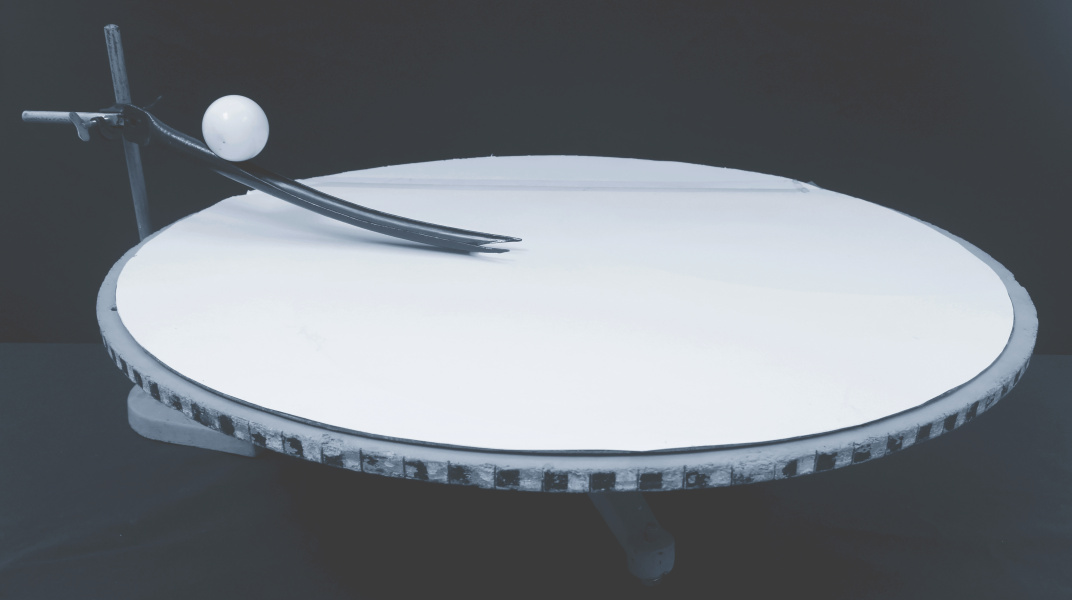
\includegraphics[width=0.8\linewidth]{Coriolis-1.png}
	\caption{Демонстрация действия силы Кориолиса на модели шара, движущегося во вращающейся системе отсчета}
	\label{Coriolis-1}
\end{figure}
	
	\subsection*{\textcolor{PineGreen}{Оборудование}}

		\begin{enumerate}
			\item Бильярдный шар, окрашенный чернилами.
			\item Наклонный желоб.
			\item Круглая платформа на вращающейся подставке.
			\item Электродвигатель с ременной передачей.
			\item Лабораторный трансформатор для регулирования скорости вращения платформы.
		\end{enumerate}

		\subsection*{\textcolor{PineGreen}{Основные определения}}
		
		Система отсчета, связанная с земным шаром, строго говоря, неинерциальная система отсчета (НИСО).
		Решения основных уравнений динамики в неинерциальных системах отсчета, в общем случае, расходятся с результатами экспериментов. Однако существует способ, используя 2 закон Ньютона, получить верный результат — ввести в рассмотрение фиктивные силы инерции в НИСО. Если сравнить решения уравнений движения для какого-либо конкретного тела, полученные в предположении, что система отсчета, связанная с Землей, инерциальная, и решения этих же уравнений с учетом сил инерции, можно обнаружить их расхождение.
		Сравнивая те и другие решения с данными опыта, можно также установить, является ли выбранная нами система инерциальной или же движется ускоренно.
		Такие проверки показали, что система координат, связанная с Землей, для большого класса механических задач может рассматриваться как инерциальная система отсчета.	
	
	
	\subsection*{\textcolor{PineGreen}{Краткое описание}}
	
Круглая платформа диаметром 100 см располагается на специальной вращающейся подставке. 
Над платформой устанавливается неподвижно небольшой наклонный желоб, с которого 
скатывается бильярдный шар (конец наклонного желоба находится над центром круга). 
Чтобы наблюдать траекторию шара, его поверхность покрывается чернилами.

\begin{figure}[H] 	
	\centering 	
	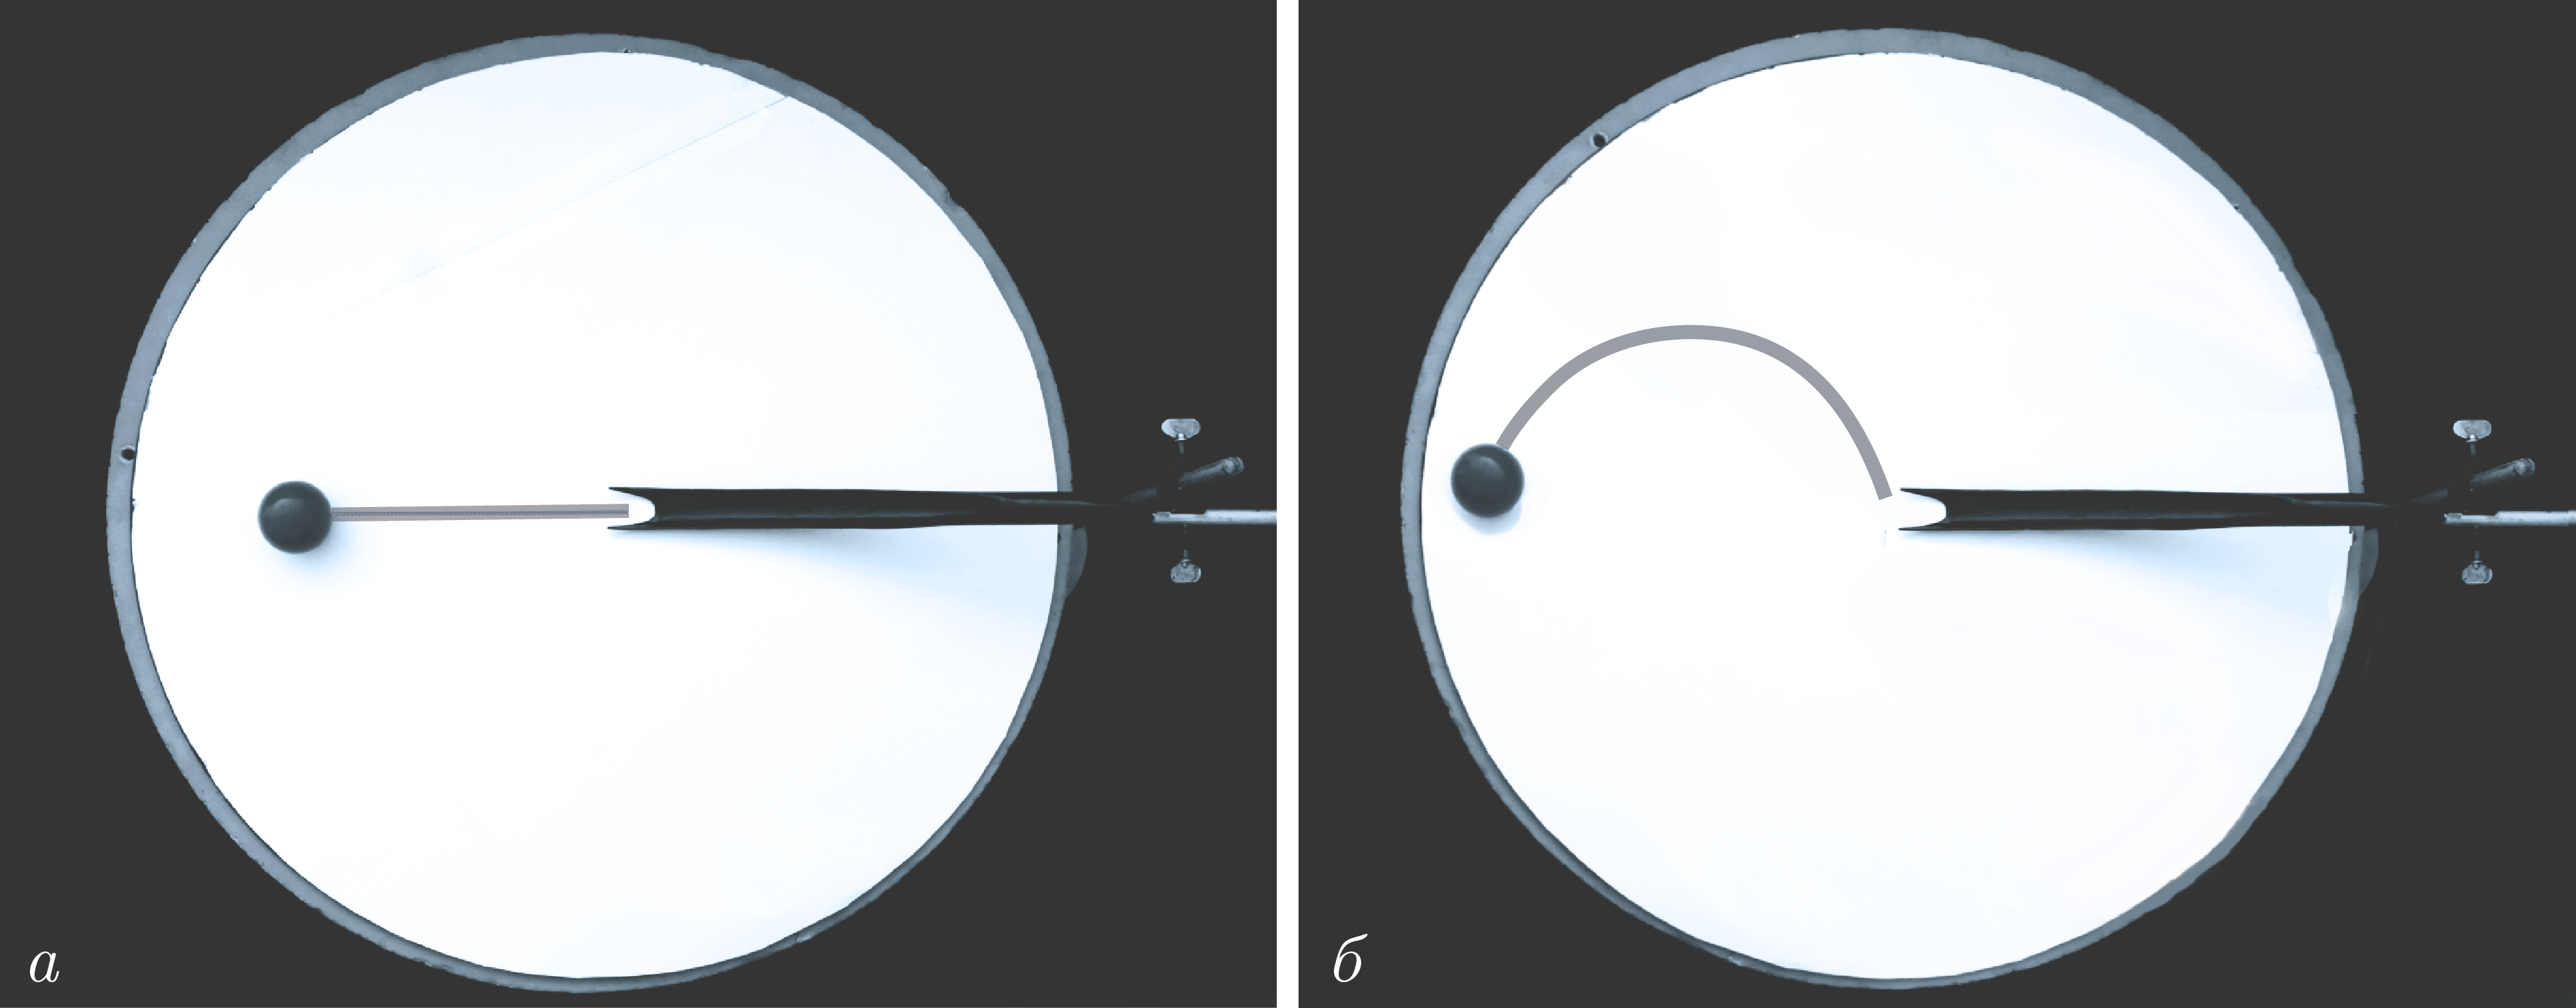
\includegraphics[width=0.9\linewidth]{Coriolis-2.png}
	\caption{\textit{а} — в отсутствие вращения платформы ($ \omega=0 $, платформа является инерциальной системой отсчета) шарик движется относительно стола по прямой линии, а вектор его скорости \textbf{v} сохраняет направление; \textit{б} — при вращении платформы на шарик начинает действовать кориолисова сила инерции, и вектор \textbf{v} изменяет направление. След, оставленный шариком на бумаге, демонстрирует траекторию движения тела относительно вращающейся системе отсчета (НИСО) , в неподвижной системе отсчета движение шарика оставалось прямолинейным}
	\label{Coriolis-2}
\end{figure}

Сначала шарик скатывают по неподвижной платформе: его траектория представлет собой прямую линию.
При медленном равномерном вращении платформы шарик отклоняется от прямолинейного пути в сторону, противоположную направлению вращения круга.
След, оставленный подкрашенным шаром, показывает, что траекторией двигающегося во вращающейся системе отсчета тела является дуга.

При вращении круга против часовой стрелки, что соответствует движению Земли 
(вследствие суточного вращения) в северном полушарии, шарик отклоняется вправо.
При вращении круга по часовой стрелке, что соответствует движению Земли в южном полушарии, шарик отклоняется влево.

Если запустить шар с периферии, то его траектория окажется в виде петли, подобно тому, какую траекторию описывает маятник Фуко над той же вращающейся платформой.
Такой опыт демонстрирует действие кориолисовой силы инерции на тела, двигающиеся в неинерциальной (вращающейся) системе отсчета.

	\subsection*{\textcolor{PineGreen}{Теория}}
	
	Во вращающейся системе отсчета на движущееся с начальной скоростью тело помимо центробежной силы инерции действует дополнительная сила инерции, называемая силой Кориолиса.

	Пусть по платформе начинает двигаться шар массой $ m $.
При его движении от центра платформы вдоль радиуса трением можно пренебречь и считать скорость постоянной.
	
Шарик, начав скатываться из центра по неподвижно платформе (рис.\ref{Coriolis-3},\textit{а}), через некоторое время окажется в точке $ A $.

	
	Если платформу раскрутить с угловой скоростью $ \omega $ (рис.\ref{Coriolis-3},\textit{б}), то к моменту достижения шариком края диска он окажется в точке $ B $.
	При движении по платформе шар вместо прямой \textit{OA} опишет дугу \textit{OB}.
	При этом в неподвижной системе отсчета на шарик не будут действовать никакие силы, кроме силы тяжести и реакции опоры, и относительно инерциальной системы его движение будет оставаться равномерным  $ \textbf{v} = $ const.
	
		\begin{figure}[H] 	
		\centering 	
		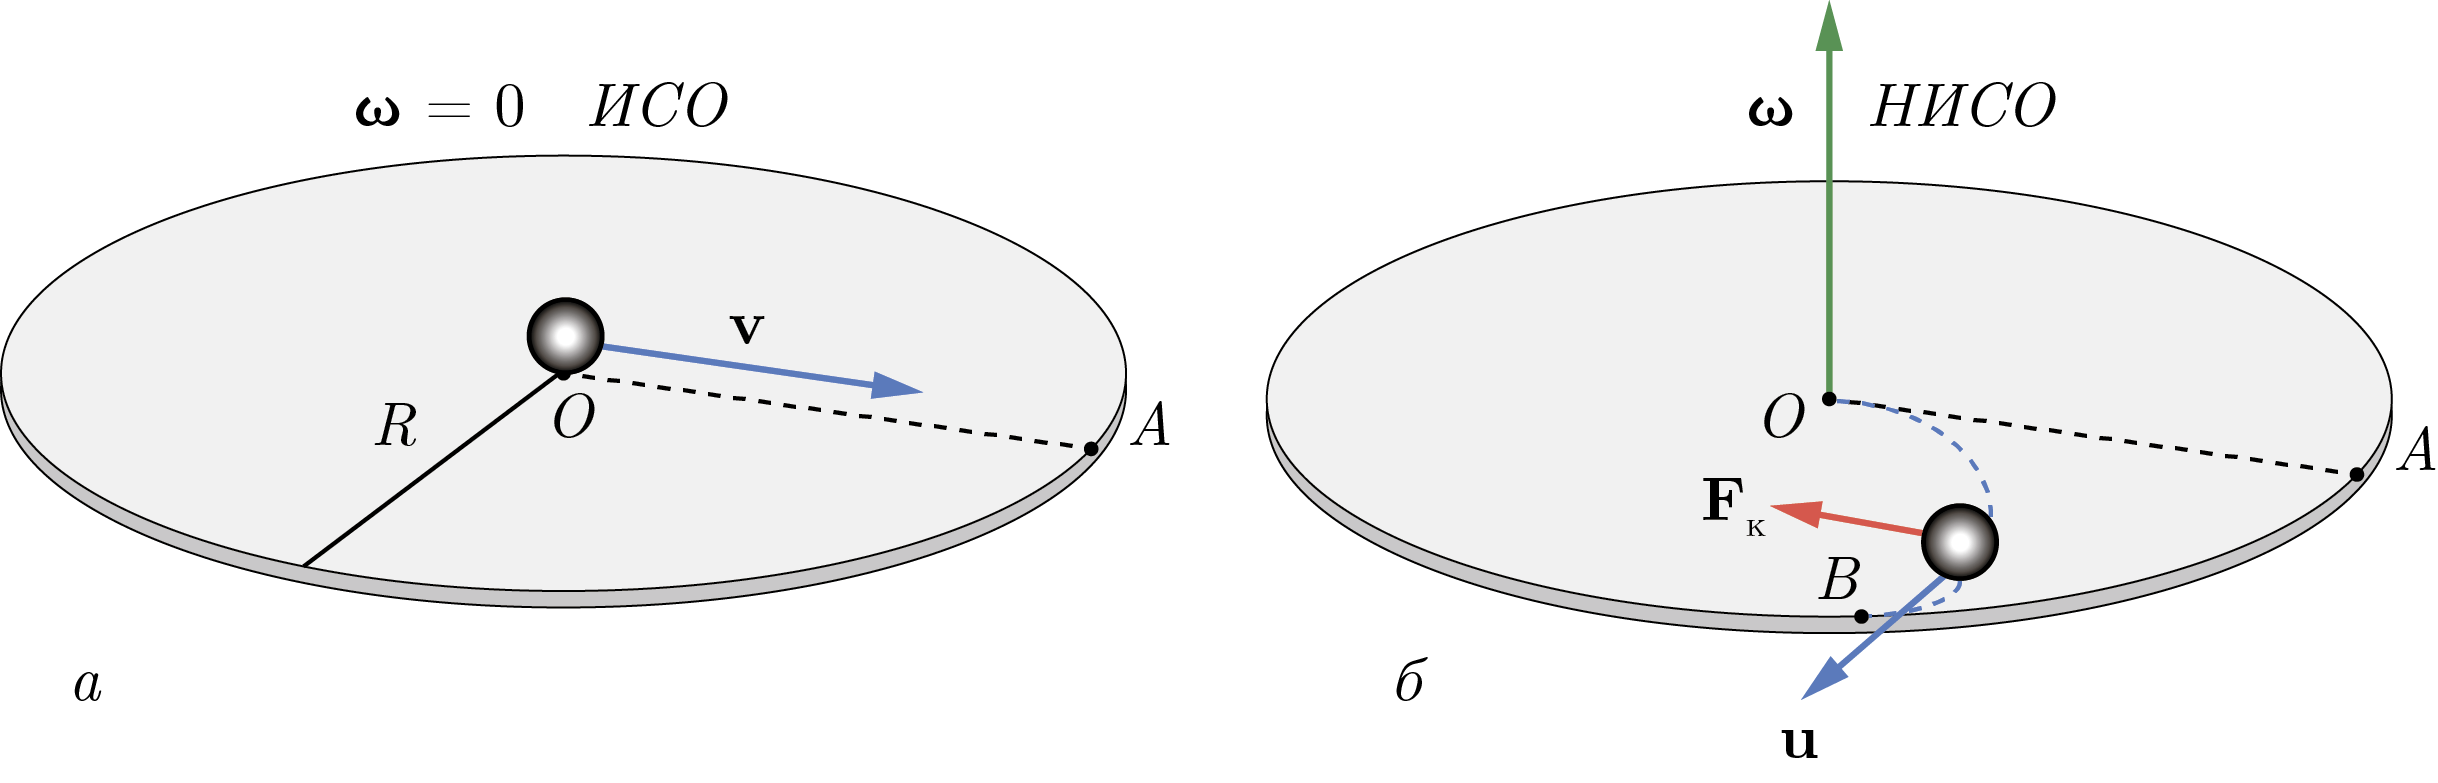
\includegraphics[width=0.9\linewidth]{Coriolis-3.png}
		\caption{Вектор скорости \textbf{v} шарика во вращающейся системе отсчета под действием силы Кориолиса будет изменять свое направление. Вращение платформы приведет к тому, что шарик, достигнув края, окажется не в точке \textit{А}, как это было бы в отсутствие вращения, а в точке \textit{В}}
		\label{Coriolis-3}
	\end{figure}

	Скорость шарика в системе отсчета, связанной с платформой, изменит направление и будет равна $ u $. Изменение скорости в НИСО объясняется проявлением инерционных свойств, в частности, на за счет действия сил инерции вектор скорости изменяет направление.
	Такая сила, меняющая направление вектора скорости тела в НИСО, но не изменяющая его модуля, называется силой Кориолиса.
	В общем виде сила Кориолиса определяется векторным произведением
	\begin{equation}\label{Coriolis-1eq5}
	\textbf{F}_{\text{К}} = 2m\textbf{u}\times\textbf{ω},	
	\end{equation}	
	где \textit{m} — масса тела, \textbf{ω} — вектор угловой скорости вращения неинерциальной системы отсчета, \textbf{u} — вектор относительной скорости движения тела в НИСО.
	Ее направление совпадает с направлением поступательного движения штопора, ручка которого поворачивается от вектора скорости \textbf{u} к вектору угловой скорости \textbf{ω}. 

\end{document}
